\section{A corrected temporal-graph reconstruction}
\label{app:graph-reconstruction}

We examine the within-repetition behavior motivating T-GRAB's
$\mathcal{P}^{\mathrm{det}}_{2,32}$ analysis \citep{dizaji2025tgrab}.
These are corrected reconstructions, not historical checkpoint replays or
all-method reproductions. Both fresh seed-0 fits use CPU FP32, 100 nodes,
hidden width 128, one layer, Chebyshev order 2 and Adam at $10^{-4}$;
chronological splits contain 40/4/4 complete 64-step periods.
The one-hour pilot ends after seven complete epochs and selects epoch 7;
a later partial epoch is excluded. A separately frozen 200-epoch fit follows
below. They share a model/graph specification, not independent seed blocks.

\begin{figure}[!htbp]
\centering
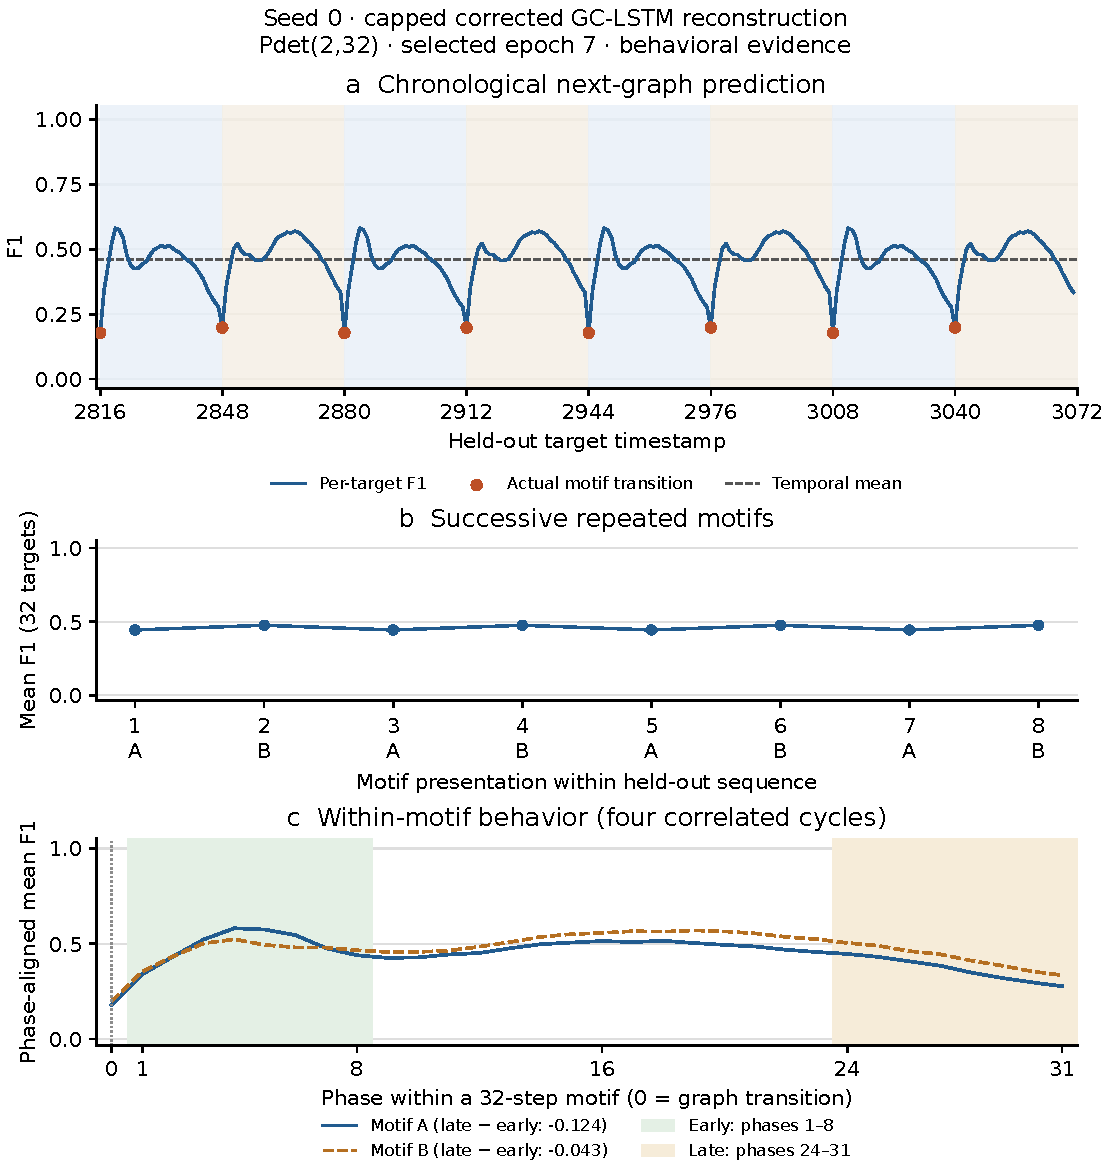
\includegraphics[width=0.90\linewidth]{figures/figure10-reconstruction.pdf}
\caption{\textbf{A capped single-model behavioral reconstruction.}
The selected model predicts all 9,900 ordered off-diagonal pairs for each
of 256 held-out targets, with probability threshold $\geq0.5$.
(a) Chronological F1; orange points mark actual graph changes, including
the first test target. (b) Means of the eight successive 32-target motif
presentations. (c) Motifs A and B aligned by within-motif phase across four
correlated cycles. The fixed early window is phases 1--8 and the late window
24--31; both exclude transition phase zero. No training-seed confidence
interval or original-paper numeric curve is shown.}
\label{fig:graph-behavior}
\end{figure}

\clearpage
\paragraph{Behavioral decline is within motifs, not cumulative across cycles.}
The held-out temporal mean F1 is 0.459277; transition and nontransition means
are 0.188305 and 0.468018. The independently verified previous-graph
persistence control averages 0.968750; the pilot curve shape therefore does
not establish strong task competence. The frozen contrast compares equal eight-phase
windows, with 32 targets per motif/window or 64 when pooling motifs.
Early and late mean F1 are 0.477737 and 0.394132 overall
(late minus early $=-0.083605$). Both motifs decline:
A, $0.488950\rightarrow0.364600$; B, $0.466524\rightarrow0.423664$.
These are descriptive window contrasts, not monotonicity claims.
The four cycles have identical per-phase confusion counts: the observed
behavior repeats rather than deteriorates cumulatively across cycles.
There is one graph realization and one trained model, not four independent
replications or evidence for an effect of periodic versus matched ordering.

\paragraph{The complete state changes the geometric interpretation.}
For the same windows, we analyze the retained pre-score states
$s_t=(h_t,c_t)\in\R^{25600}$, with canonical node order and no model rerun.
For each window we center its time cloud separately and compute FP64
sample-covariance spectra via its Gram matrix. The per-motif windows have
32 correlated rows and rank ceiling 31; pooled windows have 64 rows and
ceiling 63. Hidden-only PR falls from 1.401 to 1.053 for A and 1.397 to
1.052 for B. In contrast, \emph{complete} H+C PR rises from 1.100 to 1.292
and 1.108 to 1.231, respectively (\cref{fig:graph-state}).
Hidden-only dimensional concentration therefore does not establish a
reduction of complete-state normalized dimension.

\begin{figure}[!htbp]
\centering
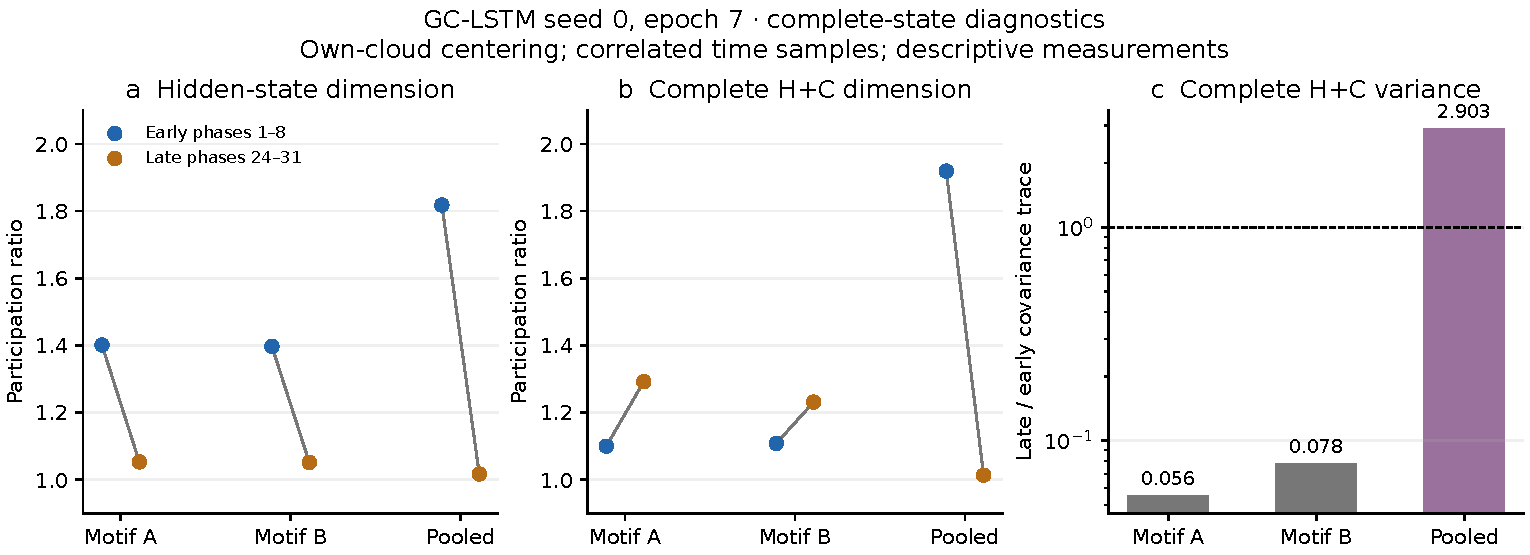
\includegraphics[width=\linewidth]{figures/figure10-state-diagnostics.pdf}
\caption{\textbf{State choice and centering qualify the behavioral observation.}
The windows and counts match \cref{fig:graph-behavior}. Hidden-only and
complete H+C participation ratios move in different directions within each
motif. Absolute covariance traces attenuate within motifs, whereas pooling
motifs mixes their different means and can increase total variance.
Late-to-early trace ratios are a post hoc display of the frozen trace
measurements, not a newly selected hypothesis test. These time-cloud
summaries have no independent-cycle confidence intervals and do not measure
causal memory or a Floquet spectrum.}
\label{fig:graph-state}
\end{figure}

Absolute covariance trace also matters: within-motif complete-state traces
fall from 8,146.28 to 452.64 for A and from 6,664.14 to 519.39 for B.
Pooling A and B instead produces a PR decrease
$1.919\rightarrow1.013$ while trace \emph{increases}
$17{,}239.60\rightarrow50{,}045.47$. The pooled cloud includes between-motif
mean separation; it is a different estimand, not corroboration of uniformly
shrinking state variance. Neither low PR nor attenuation proves loss of
useful history-dependent information.

\paragraph{Closure, verification and scope.}
Across 192 adjacent-cycle comparisons at lag 64, the maximum relative
complete-state residual is 0.005059; states are not bitwise periodic.
Identical confusion counts therefore do not imply identical states.
No periodic Jacobian or Floquet operator is certified. The runtime strictly
loads both selected weight components and verifies exact fresh train-plus-
validation H/C replay before the single held-out pass. Independent checks
verify compact metadata, spectral arithmetic, source identities and offline
W\&B transaction histories; they do not independently rerun native inference
or reanalyze the binary states. Remote dashboard delivery is unverified.
This evidence supports a within-motif behavioral decline and conditional
state-geometry diagnostics for one capped corrected GC-LSTM. It establishes
neither harmful causal retention loss, a universal collapse mechanism nor
the full multi-model, five-seed T-GRAB figure.


\clearpage
\subsection{Longer corrected fit: 200 complete epochs, selected epoch 160}
\label{app:graph-longfit}

The fresh longer fit completes 200 epochs and 511,800 optimizer updates,
stopping at its registered epoch cap; validation selects epoch 160.
It is not an extension or optimizer resume of the pilot, and the cap remains
a difference from the manuscript's stated uncapped patience policy.
The selected weights undergo exact fresh train-plus-validation H/C replay
before their single held-out evaluation. The temporal mean F1 is 0.891900;
transition and nontransition means are 0.653175 and 0.899601. This is below
the analytic persistence mean 0.968750, although persistence fails at every
transition. An aggregate ordering against that control does not identify
memory competence or a collapse mechanism.

\begin{figure}[!htbp]
\centering
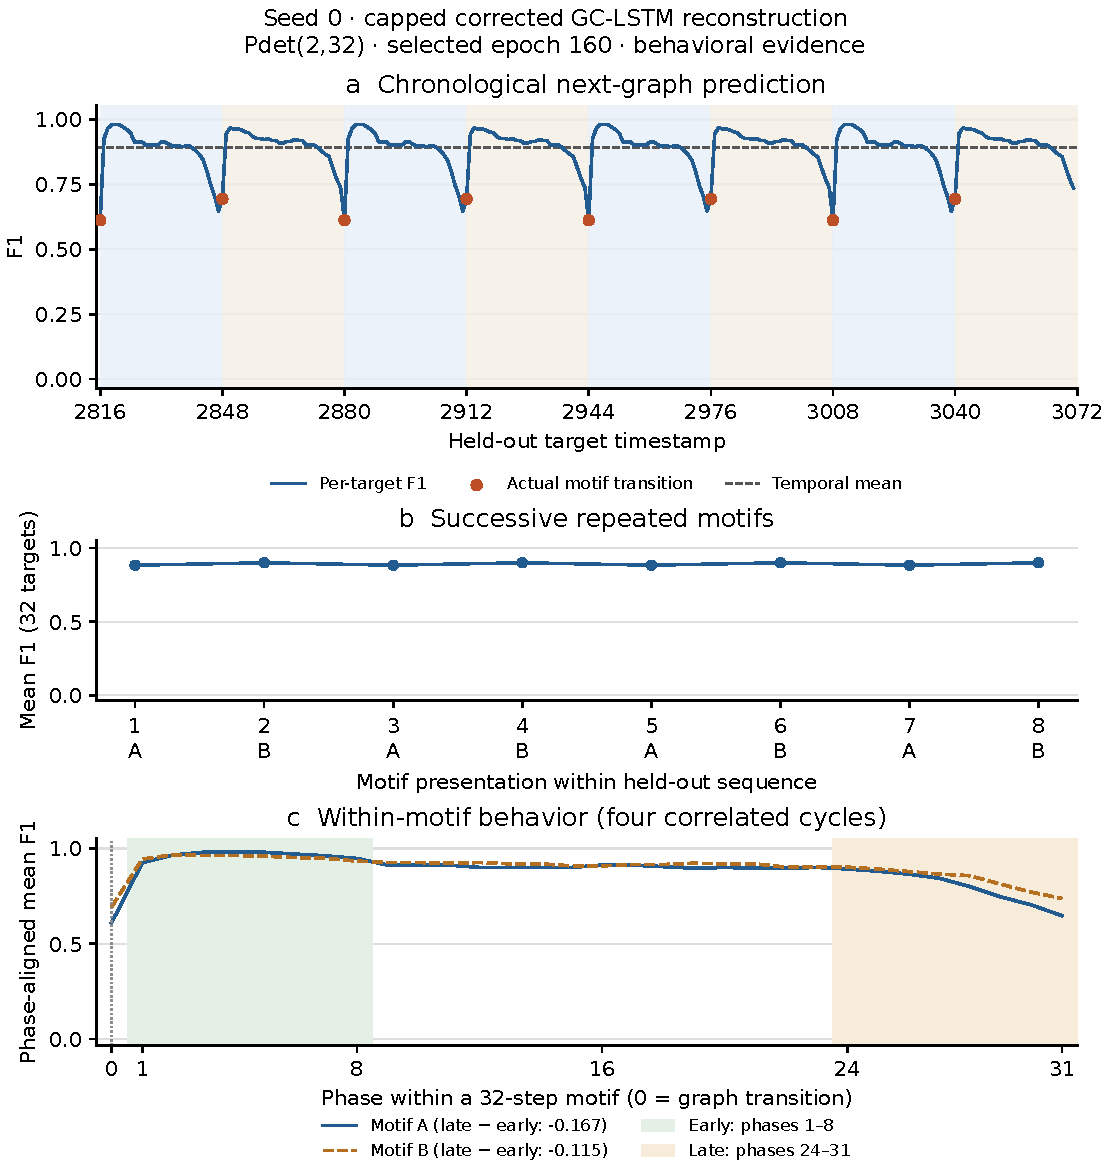
\includegraphics[width=0.90\linewidth]{figures/figure10-longfit-reconstruction.pdf}
\caption{\textbf{Behavior after the longer corrected fit.}
The same 256-target chronology, full-pair threshold rule and frozen windows
as \cref{fig:graph-behavior}, now for selected epoch 160. Both motifs have
lower late-window F1, while cycle-level means remain nearly constant.
One model seed and one graph are shown; no confidence interval, original
paper curve, monotonicity or causal retention effect is inferred.}
\label{fig:graph-longfit-behavior}
\end{figure}

\clearpage
\paragraph{The within-motif behavioral effect persists.}
For the fixed phases 1--8 versus 24--31, overall F1 decreases
$0.959297\rightarrow0.818771$ (late minus early $=-0.140526$).
Motif A decreases $0.964196\rightarrow0.797668$ and B decreases
$0.954398\rightarrow0.839874$. All four cycles have exactly matching
confusion counts and F1 at 61 of 64 aligned phases; phases 61--63 differ,
with maximum aligned F1 range 0.002749. The four cycle means lie between
0.891848 and 0.891929. This is recurring within-motif decline with small
cycle differences, not exact behavioral periodicity or cumulative decay.
The four cycles remain correlated observations from one model/graph.

\paragraph{Geometry depends on the training budget and state component.}
The complete-state PR now decreases modestly within both motifs:
$1.132672\rightarrow1.107023$ for A and
$1.128029\rightarrow1.098119$ for B. Hidden-only PR instead increases slightly
for A ($1.439486\rightarrow1.447278$) and decreases slightly for B
($1.427974\rightarrow1.419179$). These are the same own-cloud-centered
32-row windows and complete-state coordinates used above, with no estimator
or window change. The pilot's opposite hidden-versus-complete directions
therefore must not be carried over to the longer-trained weights.

\begin{figure}[!htbp]
\centering
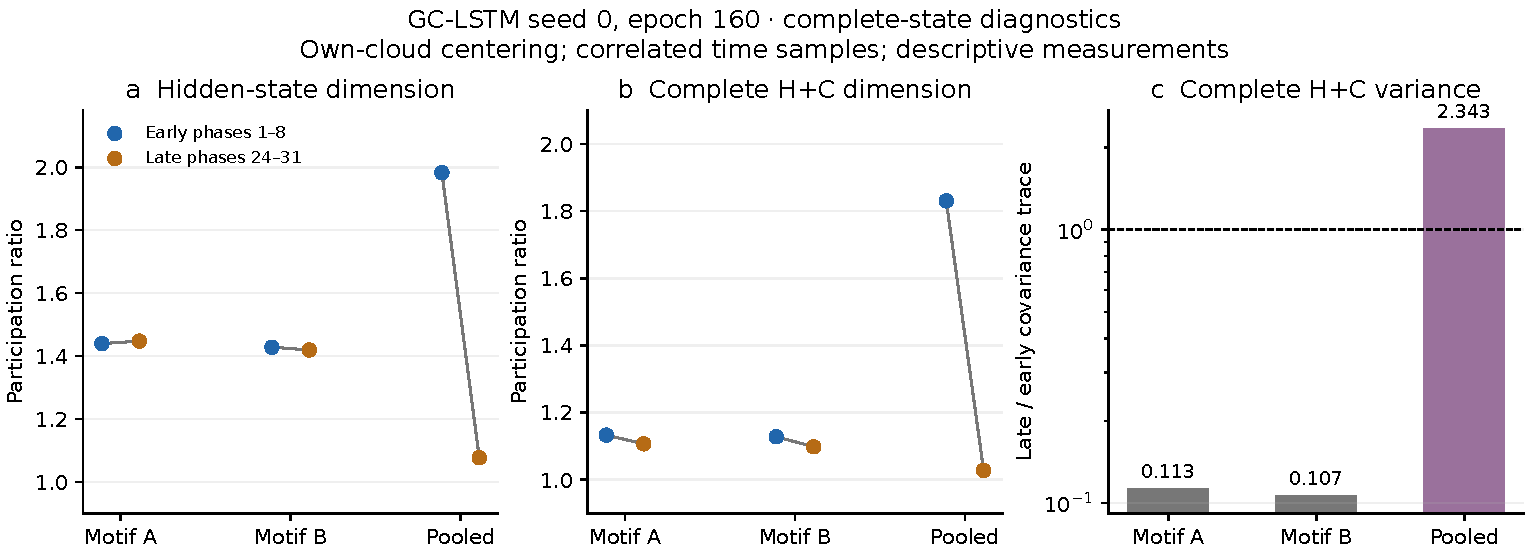
\includegraphics[width=\linewidth]{figures/figure10-longfit-state-diagnostics.pdf}
\caption{\textbf{Long-fit state geometry under the frozen analysis.}
Complete H+C PR decreases modestly in both motifs; hidden-only PR has mixed
directions. Complete covariance traces attenuate within motifs, whereas
pooling increases trace while reducing PR. Axis limits expand prospectively
to display all PR values. Ratios display frozen trace measurements;
correlated phases provide no independent-replicate interval or causal claim.}
\label{fig:graph-longfit-state}
\end{figure}

Within-motif complete covariance traces decrease
$3759.79\rightarrow423.86$ for A and $3765.73\rightarrow402.47$ for B.
Pooling motifs instead gives PR $1.830506\rightarrow1.027825$ while trace
increases $11095.62\rightarrow26000.94$. This pooled contrast includes
between-motif separation and cannot be called uniformly contracting state
variance. Covariance concentration and variance attenuation remain distinct
from loss of task-required historical information.

\paragraph{Closure and verification limit the interpretation.}
Across the same 192 lag-64 adjacent-cycle comparisons, the maximum relative
complete-state residual is 0.011679; closure is not bitwise exact. Neither
the near-repeating confusion curves nor this residual certifies periodic
Jacobians or a Floquet operator. The longer fit is Mila job 11322268
(source \texttt{1891bdd}); selected evaluation is 11330003
(\texttt{052b660}); retained-state analysis is 11330070
(\texttt{3a1a297}). Independent compact audits verify update/selection
chains, source identities, numerical summaries and actual offline W\&B
histories. They do not independently rerun inference or reanalyze raw binary
states; remote dashboard delivery remains unverified. Both training-budget
cases support a corrected single-model behavioral reconstruction and
conditional state diagnostics. Neither establishes matched-order causal
memory loss, a universal dimension-collapse mechanism or the full
multi-model, five-seed Figure 10.
